\section{}
% 3. Consider the steady flow of water through an axisymmetric garden hose nozzle 
% shown below. The axial component of velocity increases linearly from 
% 𝑢𝑧,𝑒𝑛𝑡𝑟𝑎𝑛𝑐𝑒 to 𝑢𝑧,𝑒𝑥𝑖𝑡 as sketched. Between 𝑧 = 0 and 𝑧 = 𝐿, the axial velocity 
% component is given by 𝑢𝑧 = 𝑢𝑧,𝑒𝑛𝑡𝑟𝑎𝑛𝑐𝑒 + [(𝑢𝑧,𝑒𝑥𝑖𝑡 − 𝑢𝑧,𝑒𝑛𝑡𝑟𝑎𝑛𝑐𝑒)/𝐿]𝑧. 
% Generate an expression for the radial velocity component 𝑢𝑟 between 𝑧 = 0 and 
% 𝑧 = 𝐿. You may ignore frictional effects on the walls.

Consider the steady flow of water through an axisymmetric garden hose nozzle shown below. The axial component of velocity increases linearly from $u_{z,entrance}$ to $u_{z,exit}$ as sketched. Between $z = 0$ and $z = L$, the axial velocity component is given by $u_z = u_{z,entrance} + [(u_{z,exit} - u_{z,entrance})/L]z$. Generate an expression for the radial velocity component $u_r$ between $z = 0$ and $z = L$. You may ignore frictional effects on the walls.
\begin{figure}[h]
    \centering
    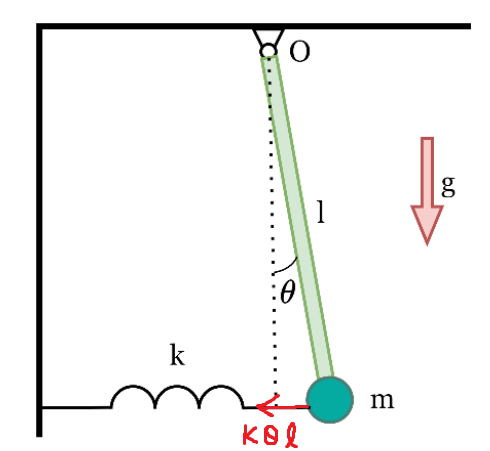
\includegraphics[width=0.5\textwidth]{Questions/Figures/q3 problem diagram.png}
    \caption{Garden hose nozzle}
\end{figure}

\subsection*{Solution}
First we list assumptions
\begin{table}
    \centering
    \caption{Assumptions}
    \begin{tabular}{c|c}
        Assumption & Approximation \\
        \hline
        Steady flow & $\partial_t = 0$ \\
        Incompressible flow & $\rho = \text{constant}$ \\
        Axisymmetric flow & $\partial_{\theta} = 0$ \\
        No friction & $\tau_{w} = 0$ \\
        No heat transfer & $q = 0$ \\
        No body forces & $\mathbf{F} = 0$ \\
    \end{tabular}
\end{table}
The continuity equation for incompressible flow is given by
\begin{align*}
    \nabla \cdot \vec{v} = 0
\end{align*}
In cylindrical coordinates, the continuity equation is given by
\begin{align*}
    \frac{1}{r}\frac{\partial}{\partial r}(r u_r) + \frac{1}{r}\frac{\partial}{\partial \theta}(u_{\theta}) + \frac{\partial}{\partial z}(u_z) = 0
\end{align*}